\setcounter{chapter}{2}
\fontsize{13}{5}\selectfont
\chapter{Phân tích hệ thống}
EHAT sẽ sử dụng các bảng có sẵn trong database của hệ thống học tập Moodle để lấy thông tin, phân tích và sẽ trả về những kết quả mà ta mong đợi. Chính vì thế nhóm chúng em sẽ nêu ra những use case cũng như những database của Moodle cần thiết phục vụ cho quá trình xây dựng công cụ EHAT.
\section{Nghiên cứu use case của hệ thống Moodle}
\subsection{Những hành động cơ bản của giáo viên và học sinh có sẵn trên Moodle}
Khi chưa thêm công cụ EHAT giáo viên và học sinh có những hành động cơ bản sau: \cite{usecase:1}
\begin{itemize}
	\item Đối với giáo viên
	\begin{center}
		\begin{figure}[htp]
			\begin{center}
				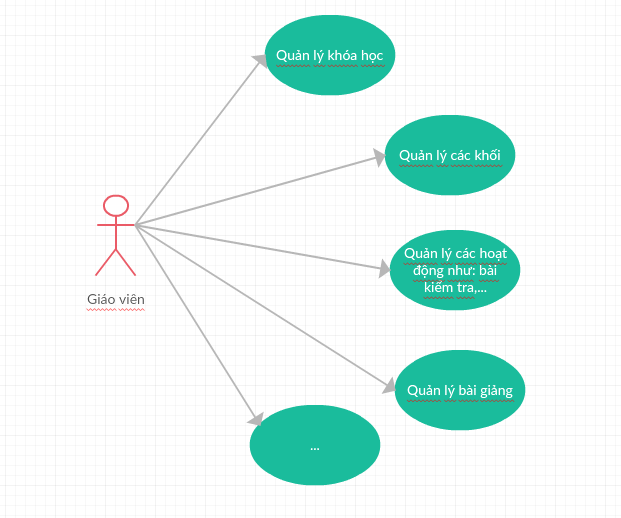
\includegraphics[scale=0.7]{img/usecasegv}
			\end{center}
			\caption{Use case thể hiện hành động cơ bản của GV}
			\label{refhinh10}
		\end{figure}
	\end{center}
	\vskip 1cm 
	\item Đối với học sinh, sinh viên
	\begin{center}
		\begin{figure}[htp]
			\begin{center}
				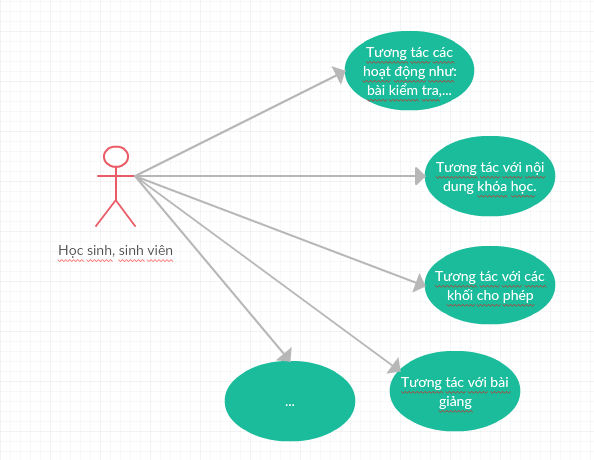
\includegraphics[scale=0.7]{img/usecasehs}
			\end{center}
			\caption{Use case thể hiện hành động cơ bản của HS, SV}
			\label{refhinh11}
		\end{figure}
	\end{center}
\end{itemize}

\subsection{Những hành động khi thêm công cụ EHAT}
Sau khi thêm vào hệ thống công cụ EHAT:
\begin{itemize}
	\item Đối với giáo viên
	\begin{center}
		\begin{figure}[htp]
			\begin{center}
				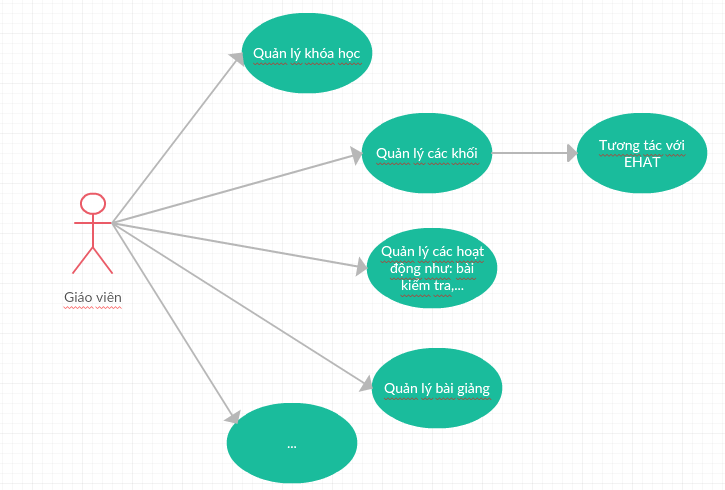
\includegraphics[scale=0.65]{img/usecasegvehat}
			\end{center}
			\caption{Use case thể hiện hành động cơ bản của GV khi có EHAT}
			\label{refhinh12}
		\end{figure}
	\end{center}
	\vskip 3cm
	\item Đối với học sinh, sinh viên
	\begin{center}
		\begin{figure}[htp]
			\begin{center}
				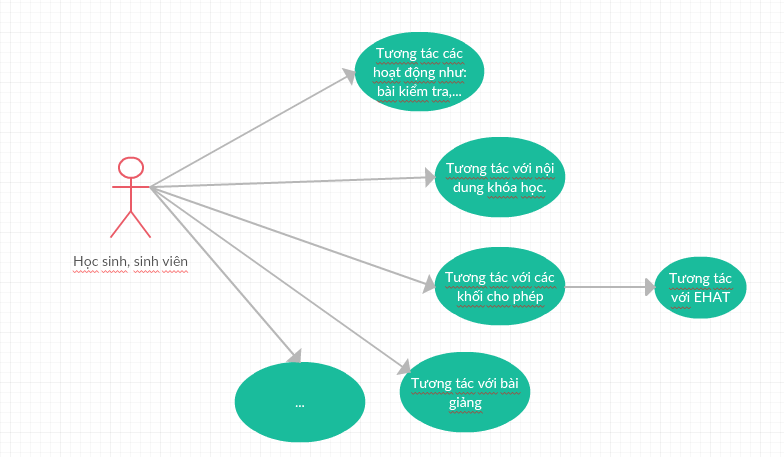
\includegraphics[scale=0.7]{img/usecasehsehat}
			\end{center}
			\caption{Use case thể hiện hành động cơ bản của HS, SV khi có EHAT}
			\label{refhinh13}
		\end{figure}
	\end{center}
\end{itemize}

Chi tiết các hoạt đông mà EHAT mang lại:
\begin{itemize}
	\item Đối với giáo viên
	\begin{center}
		\begin{figure}[htp]
			\begin{center}
				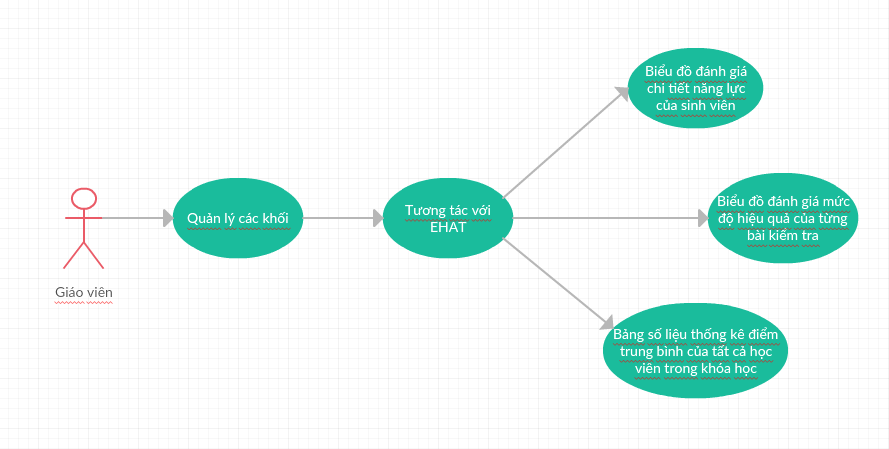
\includegraphics[scale=0.7]{img/chitietehatgv}
			\end{center}
			\caption{Các hoạt động EHAT mang lại cho GV}
			\label{refhinh14}
		\end{figure}
	\end{center}
	\vskip 4cm
	\item Đối với học sinh, sinh viên
	\begin{center}
		\begin{figure}[htp]
			\begin{center}
				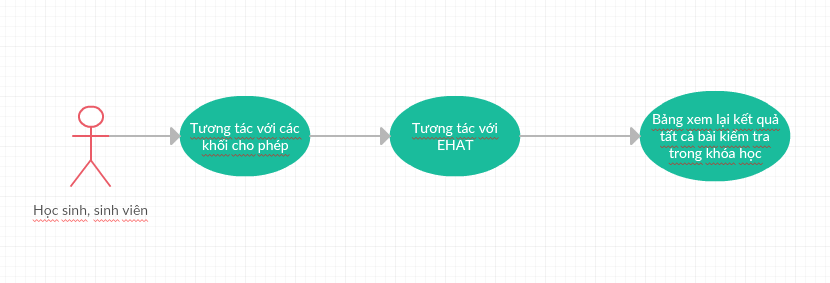
\includegraphics[scale=0.7]{img/chitietehaths}
			\end{center}
			\caption{Các hoạt động EHAT mang lại cho HS, SV}
			\label{refhinh15}
		\end{figure}
	\end{center}
\end{itemize}

\newpage
\section{Database của Moodle}

\begin{center}
	\begin{figure}[htp]
		\begin{center}
			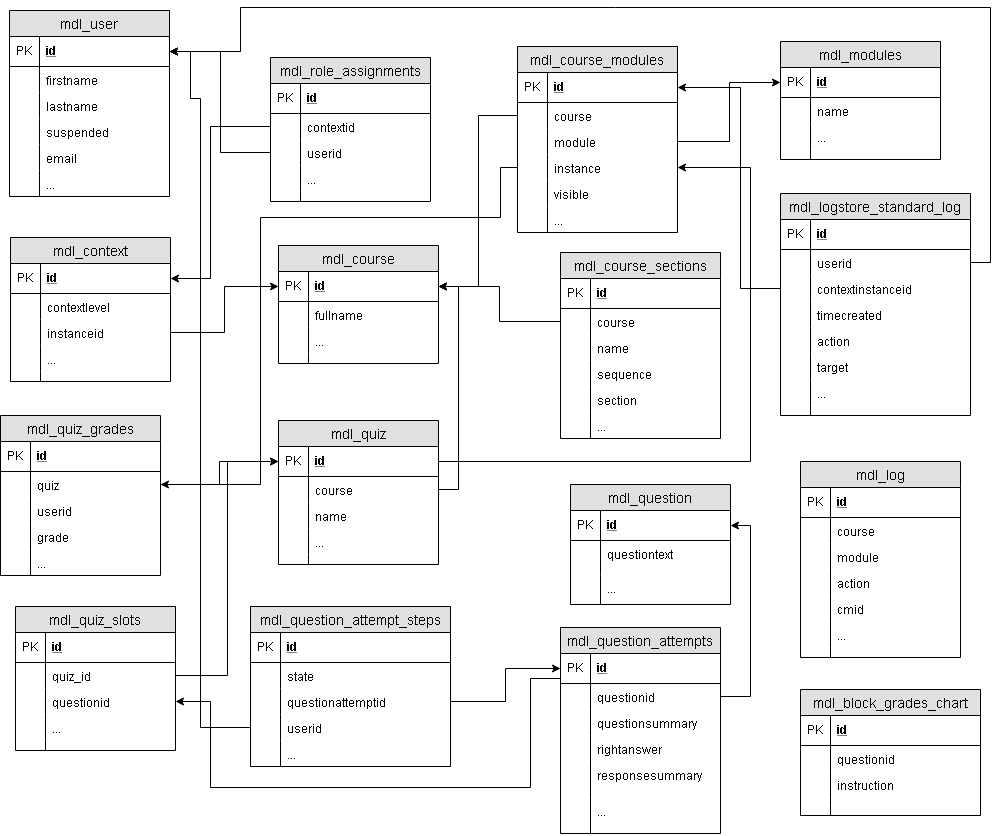
\includegraphics[scale=0.5]{img/database}
		\end{center}
		\caption{Các bảng được sử dụng}
		\label{refhinh19}
	\end{figure}
\end{center}

\newpage
Chi tiết cấu trúc cơ bản được sử dụng của từng bảng trên:
\begin{itemize}
	\item Bảng mdl\_user
	\begin{center}
		\begin{table}[!htp]
			\centering
			\begin{tabular}{|c|c|}
				\hline 
				id & Id người dùng \\ 
				\hline 
				auth &  \\ 
				\hline 
				confirmed & Kiểm tra người dùng đã được xác nhận chưa (1 hoặc 0) \\ 
				\hline 
				deleted & Xóa người dùng (1 hoặc 0) \\ 
				\hline 
				username & Tài khoản \\ 
				\hline 
				password & Mật khẩu \\ 
				\hline 
				idnumber &  \\ 
				\hline 
				firstname & Họ và lót người dùng \\ 
				\hline 
				lastname & Tên người dùng \\ 
				\hline 
				email & Email người dùng \\ 
				\hline 
				emailstop & Mặc định 0 \\ 
				\hline 
				phone1 & Số điện thoại thứ 1 \\ 
				\hline 
				phone2 & Số điện thoại thứ 2 \\
				\hline 
				address & Địa chỉ người dùng \\ 
				\hline 
				city & Thành phố \\ 
				\hline 
				country & Quốc gia \\ 
				\hline 
				lang & Ngôn ngữ \\
				\hline 
				timezone & Múi giờ \\ 
				\hline 
				firstaccess & Ngày truy cập đầu tiên \\ 
				\hline 
				lastaccess & Ngày truy cập cuối cùng \\ 
				\hline 
				lastlogin & Ngày đăng nhặp đầu tiên \\ 
				\hline 
				currentlogin & Thời gian người dùng đăng nhập hiện tại \\ 
				\hline 
				lastip & Thiết bị đăng nhập cuối cùng \\ 
				\hline 
				secret & Câu hỏi bảo mật \\ 
				\hline 
				picture & Ảnh đại diện \\
				\hline 
				description & Mô tả thông tin người dùng \\ 
				\hline 
				descriptionformat &  \\ 
				\hline 
				mailformat & HTML hoặc plaintext \\
				\hline 
				timecreated & Ngày đăng ký \\ 
				\hline 
				timemodified & Ngày chỉnh sửa \\
				\hline 
				... & ... \\
				\hline
			\end{tabular}
			\caption{Chi tiết bảng mdl\_users}
			\label{bang4}
		\end{table}
	\end{center}
	\newpage
	\item Bảng mdl\_role\_assignments
	\begin{center}
		\begin{table}[!htp]
			\centering
			\begin{tabular}{|c|c|}
				\hline 
				id & Khóa chính của bảng \\ 
				\hline 
				roleid & Khóa ngoại đến bảng role(Nơi lưu vai trò người dùng) \\ 
				\hline 
				contextid & Khóa ngoại đến bảng context \\ 
				\hline 
				userid & Id của người dùng \\ 
				\hline 
				timemodified & Thời gian chỉnh sửa bảng \\ 
				\hline 
				modifierid & Người chỉnh sửa \\ 
				\hline 
				... & ... \\
				\hline
			\end{tabular} 
			\caption{Chi tiết bảng mdl\_role\_assignments}
			\label{bang5}
		\end{table}
	\end{center}
	\item Bảng mdl\_context
	\begin{center}
		\begin{table}[!htp]
			\centering
			\begin{tabular}{|c|c|}
				\hline 
				id & Khóa chính của bảng \\ 
				\hline 
				contextlevel & Mức độ của một phạm vi trong moodle(50 là khóa học, 70 là câu hỏi,...) \\ 
				\hline 
				instanceid & Tùy thuộc vào contextlevel mà instanceid sẽ tham khảo đến \\ & id của phạm vi tương ứng \\ 
				\hline 
				... & ... \\
				\hline
			\end{tabular} 
			\caption{Chi tiết bảng mdl\_context}
			\label{bang6}
		\end{table}
	\end{center}
	\item Bảng mdl\_course
	\begin{center}
		\begin{table}[!htp]
			\centering
			\begin{tabular}{|c|c|}
				\hline 
				id & Id khóa học \\ 
				\hline 
				category &  \\ 
				\hline 
				sortorder &  \\ 
				\hline 
				fullname & Tên đầy đủ của khóa học \\ 
				\hline 
				shortname & Tên viết tắt khóa học \\ 
				\hline 
				... & ... \\
				\hline
			\end{tabular} 
			\caption{Chi tiết bảng mdl\_course}
			\label{bang7}
		\end{table}
	\end{center}
	\newpage
	\item Bảng mdl\_course\_modules
	\begin{center}
		\begin{table}[!htp]
			\centering
			\begin{tabular}{|c|c|}
				\hline 
				id & Khóa chính của bảng \\ 
				\hline 
				course & Tham khảo đến khóa học tương ứng \\ 
				\hline 
				module & Tham khảo đến mô-đun tương ứng trong Moodle \\ 
				\hline 
				instance & Tùy thuộc vào module mà instance sẽ tham khảo đến \\ & id của phạm vi tương ứng \\  
				\hline 
				visible & Điều kiện để thấy mô-đun(1: thấy, 0: ẩn) \\  
				\hline 
				... & ... \\ 
				\hline 
			\end{tabular}
			\caption{Chi tiết bảng mdl\_course\_modules}
			\label{bang8}
		\end{table}
	\end{center}
	\item Bảng mdl\_course\_sections
	\begin{center}
		\begin{table}[!htp]
			\centering
			\begin{tabular}{|c|c|}
				\hline 
				id & Khóa chính \\ 
				\hline 
				course & Liên kết đến khóa học \\ 
				\hline 
				section &  \\ 
				\hline 
				sequence & Chuỗi những mô-đun của khóa học \\ 
				\hline 
				... & ... \\ 
				\hline 
			\end{tabular} 
			\caption{Chi tiết bảng mdl\_course\_sections}
			\label{bang9}
		\end{table}
	\end{center}
	\item Bảng mdl\_quiz\_grades
	\begin{center}
		\begin{table}[!htp]
			\centering
			\begin{tabular}{|c|c|}
				\hline 
				id & Khóa chính của bảng \\ 
				\hline 
				quiz & Tham khảo đến bảng câu hỏi \\ 
				\hline 
				userid & Người dùng tương ứng \\ 
				\hline 
				grade & Điểm của người dùng \\ 
				\hline 
				timemodified & Thời gian điểm được thay đổi \\ 
				\hline 
			\end{tabular} 
			\caption{Chi tiết bảng mdl\_quiz\_grades}
			\label{bang10}
		\end{table}
	\end{center}
	\item Bảng mdl\_quiz
	\begin{center}
		\begin{table}[!htp]
			\centering
			\begin{tabular}{|c|c|}
				\hline 
				id & Id của bài kiểm tra \\ 
				\hline 
				course & Khóa học tương ứng \\ 
				\hline 
				name & Tên của bài kiểm tra \\ 
				\hline 
				... & ... \\ 
				\hline 
			\end{tabular} 
			\caption{Chi tiết bảng mdl\_quiz}
			\label{bang11}
		\end{table}
	\end{center}
	\newpage
	\item Bảng mdl\_question
	\begin{center}
		\begin{table}[!htp]
			\centering
			\begin{tabular}{|c|c|}
				\hline 
				id & Id của câu hỏi \\ 
				\hline 
				questiontext & Chi tiết câu hỏi \\ 
				\hline 
				... & ... \\ 
				\hline 
			\end{tabular} 
			\caption{Chi tiết bảng mdl\_question}
			\label{bang12}
		\end{table}
	\end{center}
	\item Bảng mdl\_quiz\_slots
	\begin{center}
		\begin{table}[!htp]
			\centering
			\begin{tabular}{|c|c|}
				\hline 
				id & Khóa chính của bảng \\ 
				\hline 
				quiz\_id & Tham khảo đến bài kiểm tra \\ 
				\hline 
				questionid & Tham khảo đến câu hỏi \\ 
				\hline 
				... & ... \\ 
				\hline 
			\end{tabular} 
			\caption{Chi tiết bảng mdl\_quiz\_slots}
			\label{bang13}
		\end{table}
	\end{center}
	\item Bảng mdl\_question\_attempt\_steps
	\begin{center}
		\begin{table}[!htp]
			\centering
			\begin{tabular}{|c|c|}
				\hline 
				id & Khóa chính của bảng \\ 
				\hline 
				state & Trạng thái của câu hỏi \\ 
				\hline 
				questionattempid & Tham khảo đến bảng questionattemps \\ 
				\hline 
				userid & Id người dùng \\
				\hline
				... & ... \\ 
				\hline 
			\end{tabular} 
			\caption{Chi tiết bảng mdl\_question\_attemp\_steps}
			\label{bang14}
		\end{table}
	\end{center}
	\item Bảng mdl\_question\_attempts
	\begin{center}
		\begin{table}[!htp]
			\centering
			\begin{tabular}{|c|c|}
				\hline 
				id & Khóa chính của bảng \\ 
				\hline 
				questionid & Tham khảo đến câu hỏi \\ 
				\hline 
				questionsummary & Chi tiết câu hỏi và câu trả lời \\ 
				\hline 
				rightanswer & Câu trả lời đúng \\
				\hline
				responsesummary & Câu trả lời của người dùng \\
				\hline
				... & ... \\ 
				\hline 
			\end{tabular} 
			\caption{Chi tiết bảng mdl\_question\_attemp}
			\label{bang15}
		\end{table}
	\end{center}
	\newpage
	\item Bảng mdl\_modules
	\begin{center}
		\begin{table}[!htp]
			\centering
			\begin{tabular}{|c|c|}
				\hline 
				id & Id của mô-đun \\ 
				\hline 
				name & Tên của mô-đun \\ 
				\hline
				... & ... \\ 
				\hline 
			\end{tabular} 
			\caption{Chi tiết bảng mdl\_modules}
			\label{bang16}
		\end{table}
	\end{center}
	\item Bảng mdl\_logstore\_standard\_log
	\begin{center}
		\begin{table}[!htp]
			\centering
			\begin{tabular}{|c|c|}
				\hline 
				id & Id của bảng \\ 
				\hline 
				userid & Id người dùng \\ 
				\hline
				contextinstanceid & Tùy thuộc vào contextlevel mà contextinstanceid \\ & sẽ tham khảo đến id của phạm vi tương ứng \\
				\hline
				timecreated & Thời gian log được tạo \\ 
				\hline
				action & Hành động của người dùng \\
				\hline 
				target & Mục đích của hành động \\
				\hline
				... & ... \\ 
				\hline 
			\end{tabular} 
			\caption{Chi tiết bảng mdl\_logstore\_standard\_log}
			\label{bang17}
		\end{table}
	\end{center}
	\item Bảng mdl\_log
	\begin{center}
		\begin{table}[!htp]
			\centering
			\begin{tabular}{|c|c|}
				\hline 
				id & Id của bảng \\ 
				\hline 
				course & Id của khóa học tương ứng \\ 
				\hline
				module & Id của mô-đun tương ứng \\
				\hline
				action & Hành động của người dùng \\
				\hline 
				cmid & Tham khảo bảng mdl\_course\_modules \\
				\hline
				... & ... \\ 
				\hline 
			\end{tabular} 
			\caption{Chi tiết bảng mdl\_log}
			\label{bang18}
		\end{table}
	\end{center}
	
	\item Bảng mdl\_block\_grades\_chart
	\begin{center}
		\begin{table}[!htp]
			\centering
			\begin{tabular}{|c|c|}
				\hline 
				id & Khóa chính của bảng \\ 
				\hline 
				questionid & Id của câu hỏi \\ 
				\hline
				instruction & Nội dung tài liệu tham khảo \\
				\hline 
			\end{tabular} 
			\caption{Chi tiết bảng mdl\_block\_grades\_chart}
			\label{bang19}
		\end{table}
	\end{center}
\end{itemize}

\newpage
\section{Những dạng biểu đồ sẽ được sử dụng trong EHAT}
EHAT sử dụng dữ liệu trong database của Moodle từ những khóa học riêng lẻ để phân tích và xây dựng các biểu đồ để thể hiện các mục tiêu mà ta mong đợi. Để đáp ứng được những mục tiêu đó với từng loại dữ liệu ta sẽ có một dạng biểu đồ tương ứng để có thể phản ảnh rõ nhất đặc điểm của dữ liệu, các dạng biểu đồ mà EHAT sử dụng bao gồm:

\begin{itemize}
	\item Biểu đồ mạng nhện (SpiderWeb)
	
	Nhóm chúng em sẽ dùng biểu đồ mạng nhện để áp dụng cho việc đánh giá và so sánh chi tiết năng lực của các HV.
	\begin{center}
		\begin{figure}[htp]
			\begin{center}
				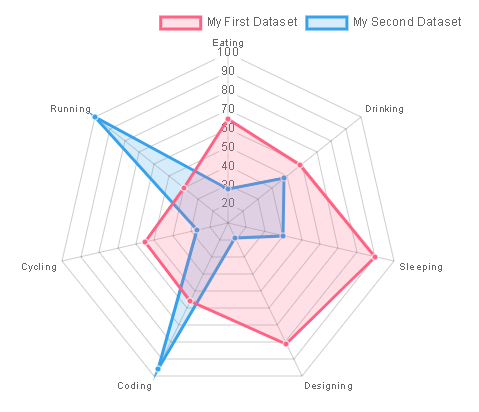
\includegraphics[scale=1]{img/radar}
			\end{center}
			\caption{Biểu đồ mạng nhện}
			\label{refhinh16}
		\end{figure}
	\end{center}
	
	\newpage
	\item Biểu đồ cột ngang (Basic bar)
	
	Biểu đồ cột ngang sẽ được áp dụng cho việc thống kê số lượng truy cập của sinh viên dựa vào những hành động mà ta muốn phân tích(VD: Số lượng sinh viên truy cập của tất cả bài kiểm tra,...).
	
	\begin{center}
		\begin{figure}[htp]
			\begin{center}
				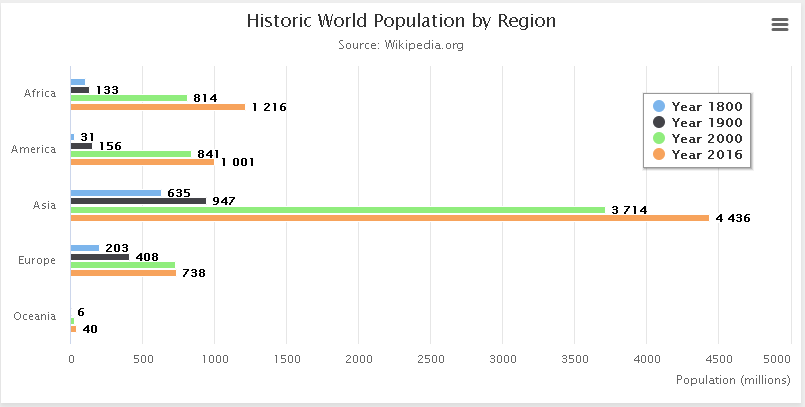
\includegraphics[scale=0.7]{img/bar}
			\end{center}
			\caption{Biểu đồ cột ngang}
			\label{refhinh17}
		\end{figure}
	\end{center}
	
	\item Biểu đồ đường (Line Chart)
	
	Biểu đồ đường được sử dụng cho việc tham khảo sự phân phối số lượt truy cập của từng sinh viên trong khóa học.
	
	\begin{center}
		\begin{figure}[htp]
			\begin{center}
				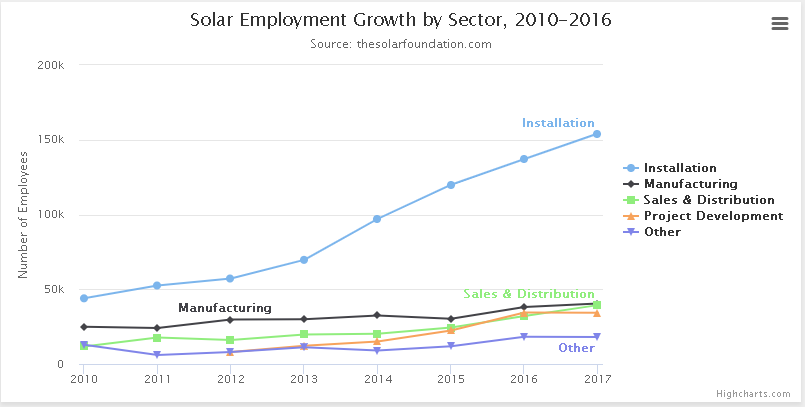
\includegraphics[scale=0.7]{img/line}
			\end{center}
			\caption{Biểu đồ đường}
			\label{refhinh18}
		\end{figure}
	\end{center}
	
\end{itemize}
